\chapter{Arbeitsergebnisse}
\begin{itemize}
	\item Ergebnisse, welche für den weiteren Verlauf relevant sind (z.B. zu realisierende Szenarien)
	\item weiterverfolgte Szenarien
\end{itemize}

\section{Szenarien}

\subsection{Effizienz und Komfort - Erkennung der Anzahl der Personen in einem Raum}
\emph{(von Philip Laube)}
\subsubsection{Ablauf}
Person A geht zusammen mit Person B vom Flur in das Wohnzimmer, während Person C in die Küche geht.
Die Lichter werden im Flur deaktiviert, im Wohnzimmer und in der Küche aktiviert.
Person D betritt die Wohnung und wird von den Personen A und B in der Tür zum Wohnzimmer begrüßt. Zusammen gehen sie ins Wohnzimmer.
Dabei werden zunächst die Lichter im Flur erneut aktiviert und nach der Begrüßung wieder deaktiviert.
Nach einiger Zeit ruft Person D zum Essen und es verlassen Personen A, B und C das Wohnzimmer und gehen in die Küche.
Sobald die letzte Person das Wohnzimmer verlassen hat werden die Lichter im Wohnzimmer deaktiviert.

\subsubsection{Erforderliche Komponenten}
\begin{itemize}
	\item ZWay Steuereinheit
	\item 2 x Bewegungsmelder / Fibaro 6-in-1 Sensor pro Tür
	\item Modul zur Lichtersteuerung
\end{itemize}

\subsubsection{zur Diskussion}
Unbekannt ob Begrüßungssituation ausreichend abgegrenzt werden kann, ohne Fehler hervorzubringen.
Tür könnte zusätzlich mit Türsensor ausgestattet werden um ein Durchgehen zu bestätigen bzw. vorbeigehende Personen bei geschlossener Tür zu ignorieren.

\subsubsection{Modellierung Erkennung der Personenanzahl}
%TODO textuelle Beschreibung der Modelle
\emph(//TODO BITTE NOCH BESCHREIBUNGSTEXT EINFÜGEN (siehe Modell))
\begin{figure}[h!]
	\centering
	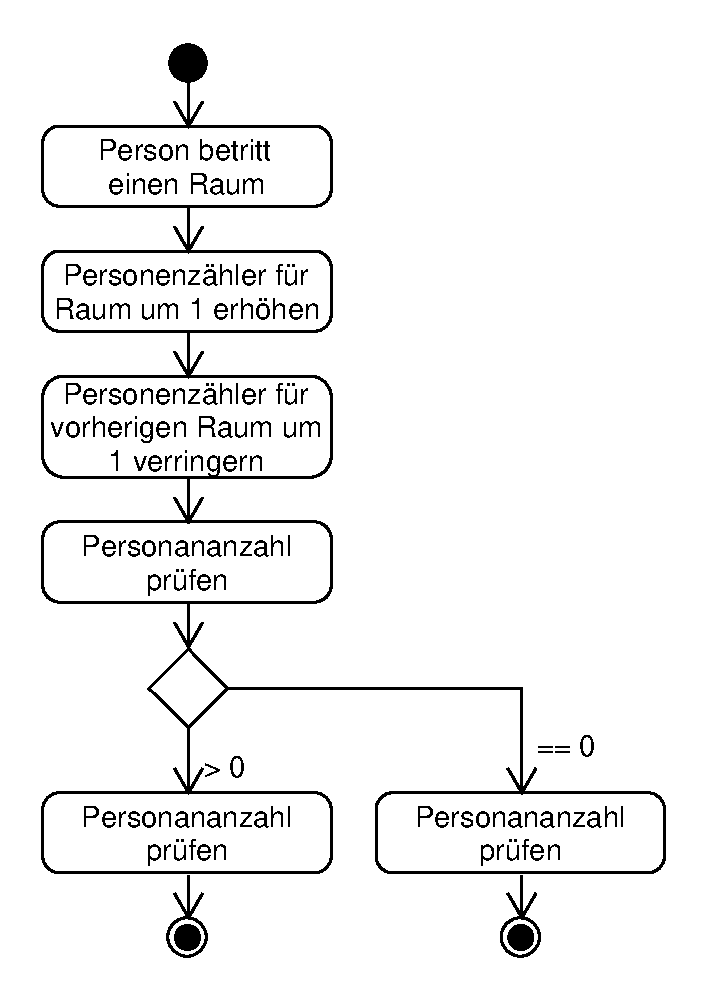
\includegraphics[scale=0.8]{img/Szenarien/ErkennungAnzahlPersonen.pdf}
	\caption{Erkennung der Personenanzahl}
	\label{fig:szenarienPersonenerkennung}
\end{figure}

\subsubsection{Modellierung Personenerkennung an der Tür}
\emph(//TODO BITTE NOCH BESCHREIBUNGSTEXT EINFÜGEN (siehe Modell))
\begin{figure}[h!]
	\centering
	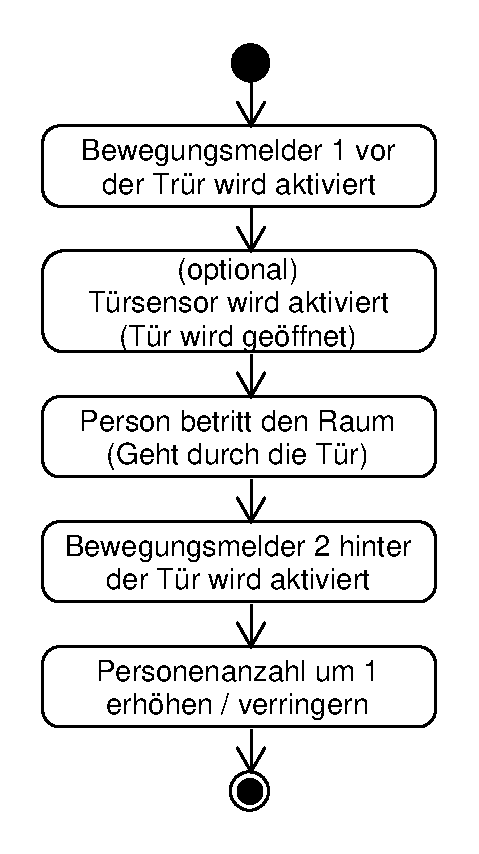
\includegraphics[scale=0.8]{img/Szenarien/PersonenerkennungAnTuer.pdf}
	\caption{Personenerkennung an der Tür}
	\label{fig:szenarienPersonenerkennungTür}
\end{figure}

\subsection{Haus bei verschließen der Haus- Wohnungstür in "`Standby"' versetzen}
\emph{(von Simon Schwabe)}
\subsubsection{Ablauf}
Um den Komfort in ihrem Smart Home zu steigern, möchte Anne möglichst wenig Aufwand zur Steuerung des Lichts betreiben. Dazu möchte sie bei Verlassen der Wohnung nicht alle angeschalteten Lampen manuell ausschalten und überprüfen, ob Gefahrenquellen vom Stromnetz getrennt sind.

Ein intelligentes, vernetztes Türschloss überträgt dazu beim Abschließen der Wohnung ein entsprechendes Signal an die zentrale Steuereinheit. Diese Steuereinheit interpretiert das Signal und schaltet alle Lampen aus. Außerdem werden vorher konfigurierte Steckdosen deaktiviert, um das Brandrisiko zu minimieren. Damit wird die Wohnung in einen "`Standby-Modus"' versetzt. Auch in diesem Fall möchte Anne nicht alle Geräte vom Stromnetz trennen, ihr Laptop soll weiterhin mit Strom versorgt und der Akku geladen werden.

Befindet sich Tom noch in der Wohnung, wenn sie abschließt, soll er nicht durch die Steuerung gestört werden. Das heißt in diesem Fall wird die automatische Abschaltung nicht durchgeführt. Dazu ist es notwendig, dass verschiedene Sensoren des Systems zuverlässig erkennen, ob Personen anwesend sind. Die automatische Steuerung wird erst aktiv, wenn der letzte Bewohner die Wohnung verlässt und abschließt.

Der Standby-Modus wird mit Aufschließen der Wohnungstür deaktiviert. Es erscheint allerdings nicht sinnvoll, den Zustand zum Zeitpunkt des Verlassens wiederherzustellen, da die Anforderungen an Beleuchtung usw. beim Ankommen grundlegend andere als bei Verlassen der Wohnung sein können. Diese sind abhängig von der Tageszeit.

\subsubsection{zur Diskussion}
\begin{itemize}
	\item welche Komponenten sind von Abschaltung betroffen (z.B. Lampen, Steckdosen von Wasserkocher, Kaffeemaschine, ...)
	\item welche Komponenten sind ausgeschlossen (z.B. Kühl- und Gefrierschränke, Waschmaschinen, ...)
\end{itemize}

\subsubsection{erforderliche Komponenten}
\begin{itemize}
	\item Steuereinheit
	\item vernetztes Türschloss
	\item Sensoren zu Personenerkennung: z.B. Bewegungsmelder, Infrarot
	\item schaltbare Steckdosen, evtl. mit Verbrauchserkennung
	\item schaltbare Lampen
\end{itemize}


\subsubsection{Modellierung aus Nutzersicht}
Das Modell (\prettyref{fig:szenarienStandbyNutzersicht}) verdeutlicht die im Szenario beschriebene Interaktion des Nutzers mit dem System. Ziel des Szenarios ist es, dem Nutzer möglichst hohen Komfort zu bieten. Aus diesem Grund sind die Interaktionsmöglichkeiten des Nutzers mit dem System bewusst auf das Notwendigste beschränkt. Das Szenario wird indirekt durch den Nutzer initiiert, indem er die Wohnungstür abschließt. Auf diese Weise entsteht für die Nutzer kein Mehraufwand und keine direkte Interaktion mit dem System.

Mit dem Abschließen der Tür ist die Erwartung des Nutzers verbunden, dass die Wohnung in einen Standby-Modus tritt. Sollte dies aufgrund anwesender Personen nicht möglich sein, sollte der Nutzer über ein geeignetes Mittel darüber informiert werden. Dazu kann beispielsweise eine Benachrichtigung auf das Mobiltelefon des Nutzers gesendet werden.

\begin{figure}[h!]
	\centering
	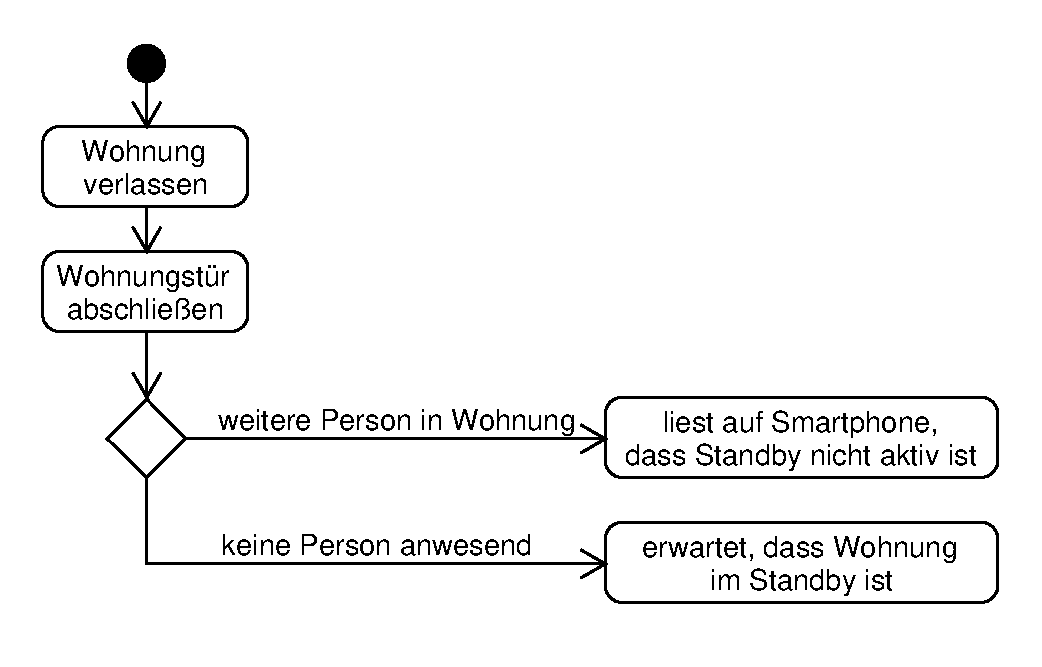
\includegraphics[width=0.9\textwidth]{img/Szenarien/WohnungSchliessenNutzersicht.pdf}
	\caption{Abläufe bei Verschließen der Wohnung aus Nutzersicht}
	\label{fig:szenarienStandbyNutzersicht}
\end{figure}

\subsubsection{Modellierung aus Systemsicht}
Die technische Modellierung (\prettyref{fig:szenarienStandby}) gestaltet sich etwas umfangreicher. Gestartet wird der Ablauf durch das Schließen des konfigurierten Schlosses. Alternativ kann auch ein Schalter an der Wohnungstür betätigt werden. Das System überprüft daraufhin, ob noch Personen in der Wohnung anwesend sind. Ist das der Fall, wird die Aktion abgebrochen und anwesende Personen werden nicht in ihren Aktivitäten beeinträchtigt. In diesem Fall kann der Nutzer, welcher die Wohnung verlassen hat, informiert werden.

Wird zum Zeitpunkt des Abschließens keine anwesende Person erkannt, wird ein Timer gestartet. So lange dieser Timer aktiv ist, wird in regelmäßigen Abständen überprüft, ob Personen, bzw. Bewegungen in der Wohnung erkannt werden. Dieses Vorgehen soll die Gefahr reduzieren, dass anwesende Personen nicht wahrgenommen werden. Wird während der Laufzeit des Timers eine Person erkannt, wird die Aktion wie oben beschrieben abgebrochen.

Trotz dieses Vorgehens ist nicht auszuschließen, dass Personen in der Wohnung nicht korrekt erkannt werden. Für diesen Fall kann ein zusätzlicher Feedback-Modus implementiert werden, in dem die anwesenden, nicht erkannten Personen über die anstehende Aktion informiert werden. Erfolgt kein Feedback, werden konfigurierte Geräte in den Standby-Modus versetzt.

\begin{figure}[h!]
	\centering
	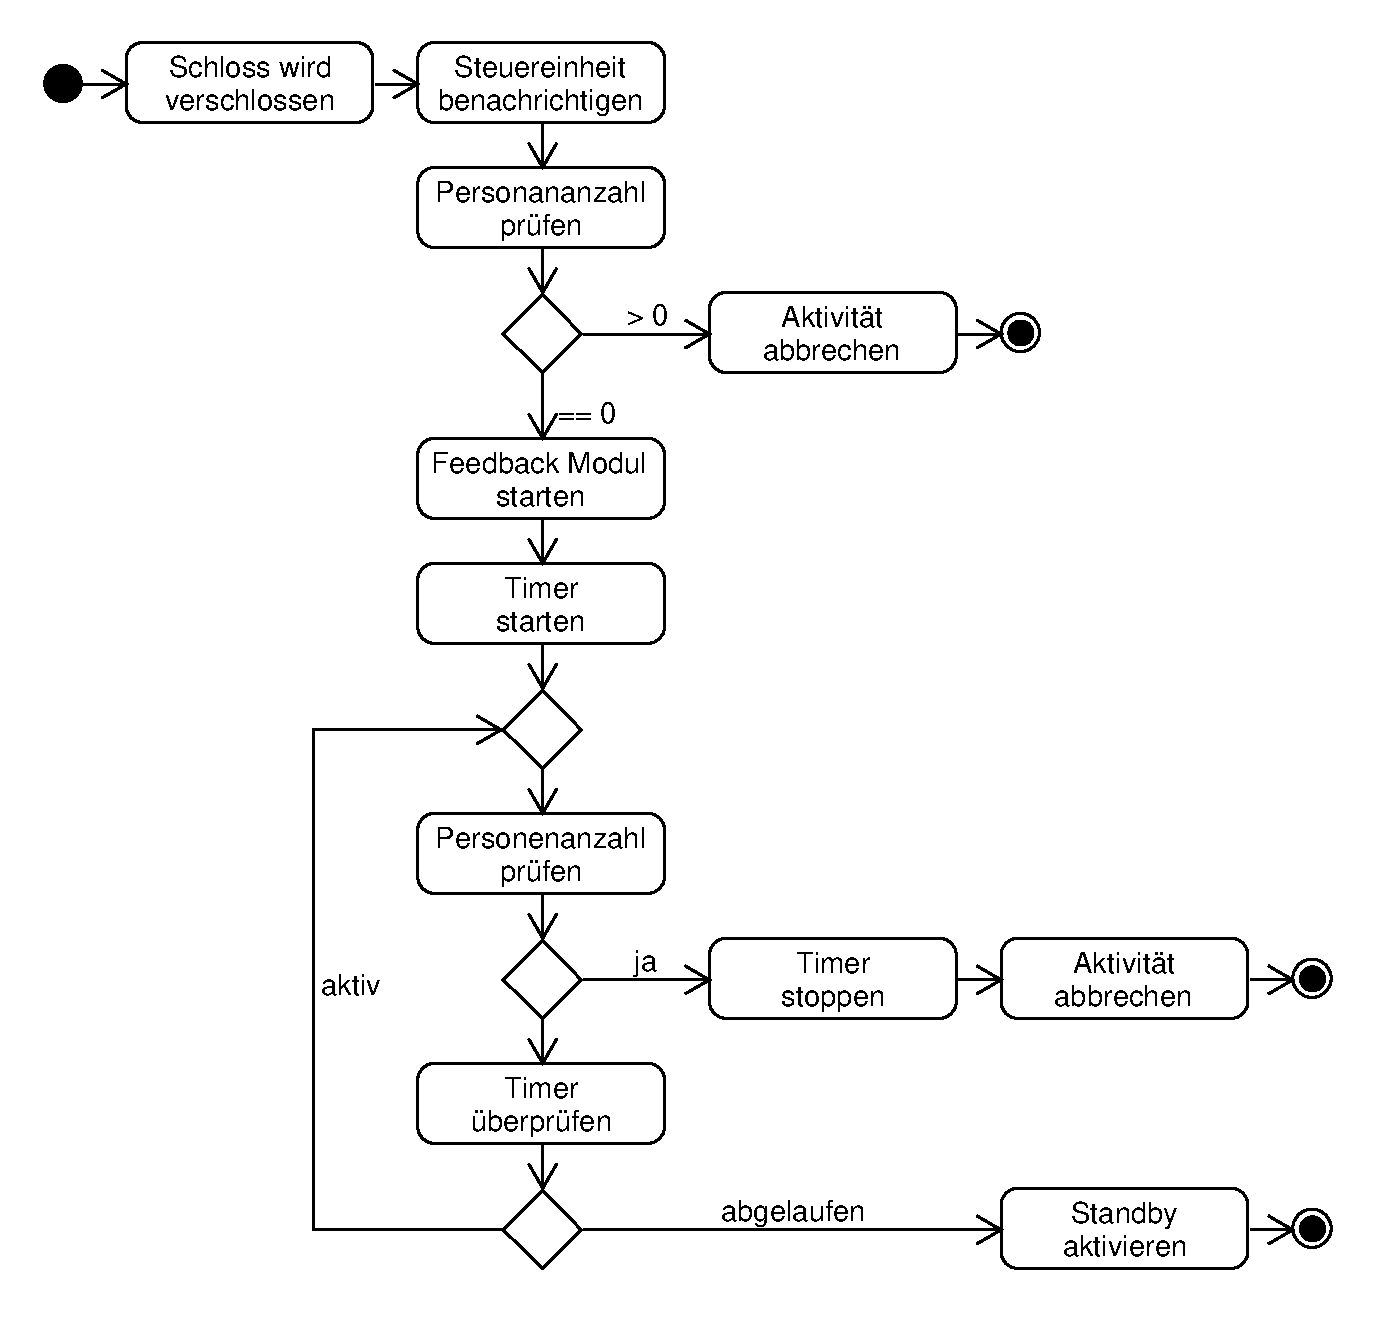
\includegraphics[width=0.9\textwidth]{img/Szenarien/WohnungSchliessen.pdf}
	\caption{Abläufe bei Verschließen der Wohnung aus Systemsicht}
	\label{fig:szenarienStandby}
\end{figure}

\subsection{Gefahrenquellen abstellen (Fibaro, CO$_2$)}
\emph{(von Martin Petzold)}
\subsubsection{Auslöser (opt.)}
\begin{itemize}
	\item Erkennung Erwachsene Person (Fibaro, CO$_2$)
\end{itemize}

\subsubsection{Vorbedingung}
\begin{itemize}
	\item Zuverlässige Erkennung ob Personen den Raum betreten oder Verlassen wurde bereits realisiert (Szenario Herr Laube)
\end{itemize}

\subsubsection{Ablauf}
Das System befindet sich im Standby, d.h. alle Gefahrenquellen im Raum sind ausgeschaltet. Person X (ein Kind) betritt den Raum. Das Betreten des Raumes wir vom System erkannt, nun wird ein Vorgang gestartet der die Person als Kind oder Erwachsenen zu identifizieren. Person X wir dabei als Kind identifiziert somit bleiben die Gefahrenquellen abgeschaltet. 
Nun betritt Person Y (ein Erwachsener) den Raum, dessen Betreten wird ebenfalls vom System erkannt. Der Erkennungsvorgang wird ein zweites mal Gestartet. das System erkennt das es sich bei einer der Beiden Personen um eine Erwachsene Person handeln muss und Schaltet die Gefahrenquellen frei so das diese benutzt werden können.
Nach einer Weile verlässt Person Y den Raum, das System Stellt fest das sich kein erwachsener mehr im Raum befindet und schaltet nach einer gewissen Zeit den Standby Modus wieder her.

\subsubsection{Alternativer Ablauf}
Nur Person Y(ein Erwachsener)  betritt den Raum, System erkennt den Eintritt. Er wird beim Identifizierungsvorgang als Erwachsener erkannt und damit werden die Gefahrenquellen freigeschaltet.
Nach einer Weile verlässt Person Y den Raum, das System Stellt fest das sich kein erwachsener mehr im Raum befindet und schaltet nach einer gewissen Zeit den Standby Modus wieder her.

\subsubsection{erforderliche Komponenten}
\begin{itemize}
	\item Fibaro 6 in 1 Sensor
	\item CO$_2$ Sensor
	\item Z-Way-Server/Steuereinheit
	\item 2 Bewegungsmelder zur Erkennung von Eintritt in den Raum
	\item Schaltbare Gefahrenquelle (zur Demonstration reicht auch eine Schaltbare Signalquelle)
\end{itemize}

\subsubsection{Nachbedingung (opt.)}
\begin{itemize}
	\item Das System kann auch eine Regelung beinhalten das der Standby Modus irgendwann automatisch und nicht nach verlassen des Raumes Zeitgesteuert wieder hergestellt wird.
\end{itemize}

\subsubsection{zur Diskussion}
\begin{itemize}
	\item Abgleich mit dem Szenario zur Erkennung  Person hat den Raum betreten/verlassen
	\item sind die Sensoren Präzise genug um den Unterschied Kind Erwachsener zu erfassen, oder kann wie im Werbevideo nur Mensch und Haustier unterschieden werden
	\item soll die Wieder Standby Schaltung des Systems Teil des Szenarios sein
	\item Einordnung in Umsetzbar/Nicht Umsetzbar
\end{itemize}

\subsubsection{ähnliche Szenarien}
\begin{itemize}
	\item Verknüpfung mit zur Erkennung  Person hat den Raum betreten/verlassen
	\item Verknüpfung mit Haus bei verschließen der Haus- Wohnungstür in "`Standby"' versetzen als Regelung zur Herstellung des Standby Zustandes
\end{itemize}

\subsubsection{Modellierung Identifizierung Erwachsener}
\emph(//TODO BITTE NOCH BESCHREIBUNGSTEXT EINFÜGEN (siehe Modell))
\begin{figure}[h!]
	\centering
	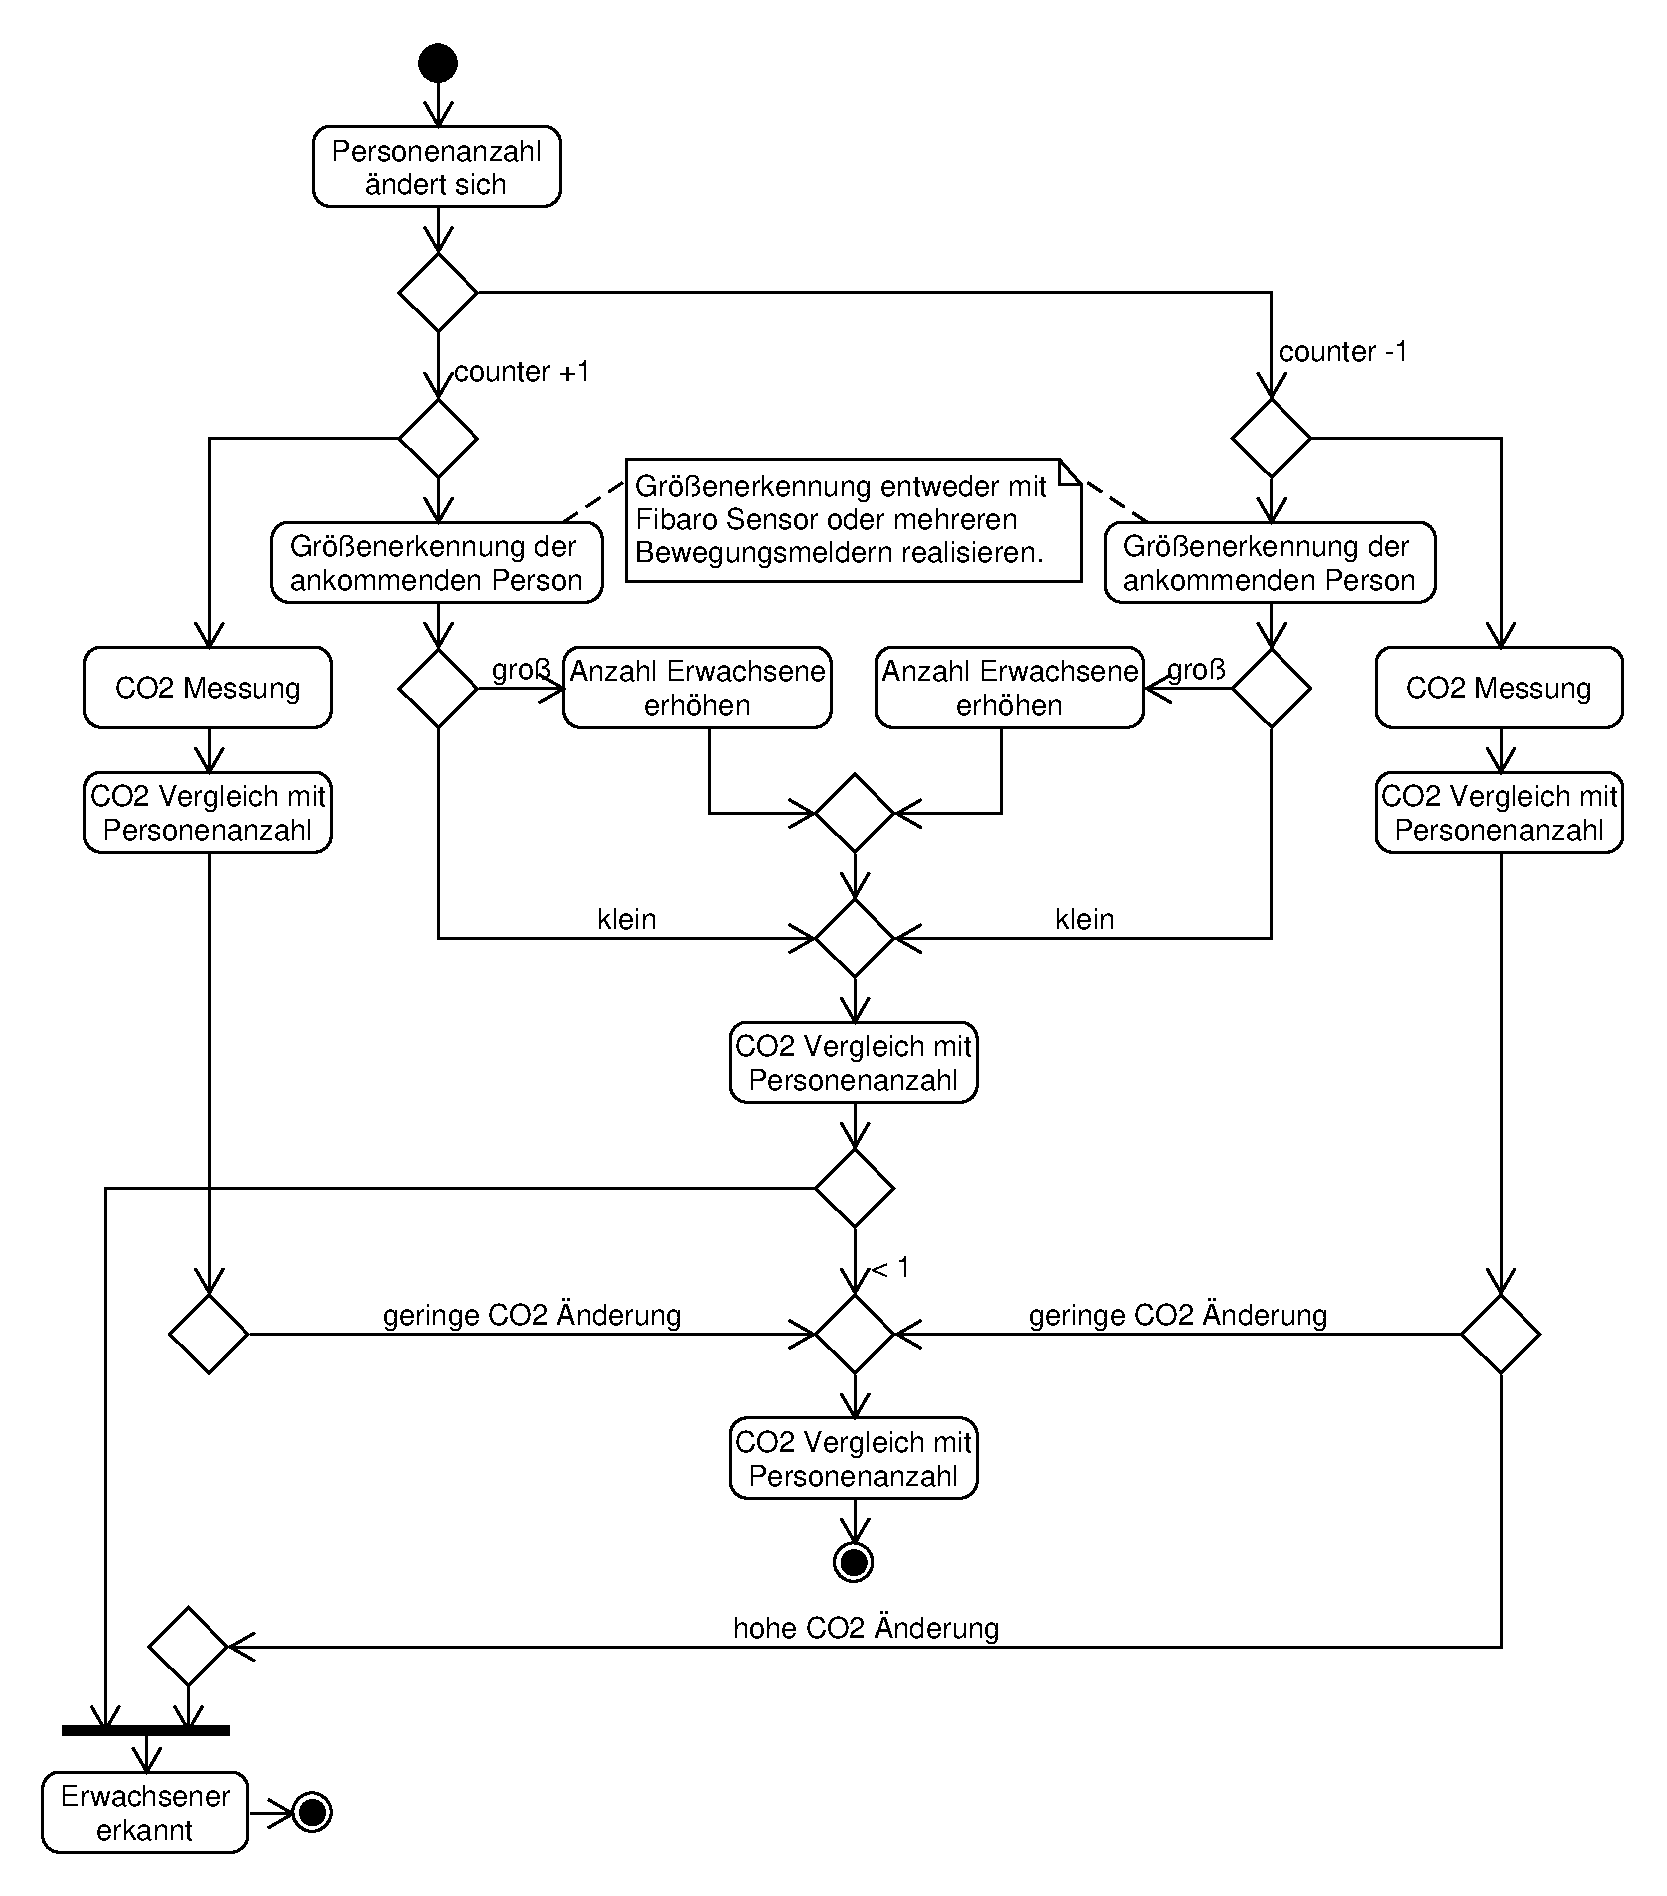
\includegraphics[width=0.9\textwidth]{img/Szenarien/IdentifizierungErwachsene.pdf}
	\caption{Identifizierung Erwachsener}
	\label{fig:szenarienIdentifizierungErwachsene}
\end{figure}

\subsubsection{Modellierung Gefahrenquellen abstellen}
\emph(//TODO BITTE NOCH BESCHREIBUNGSTEXT EINFÜGEN (siehe Modell))
\begin{figure}[h!]
	\centering
	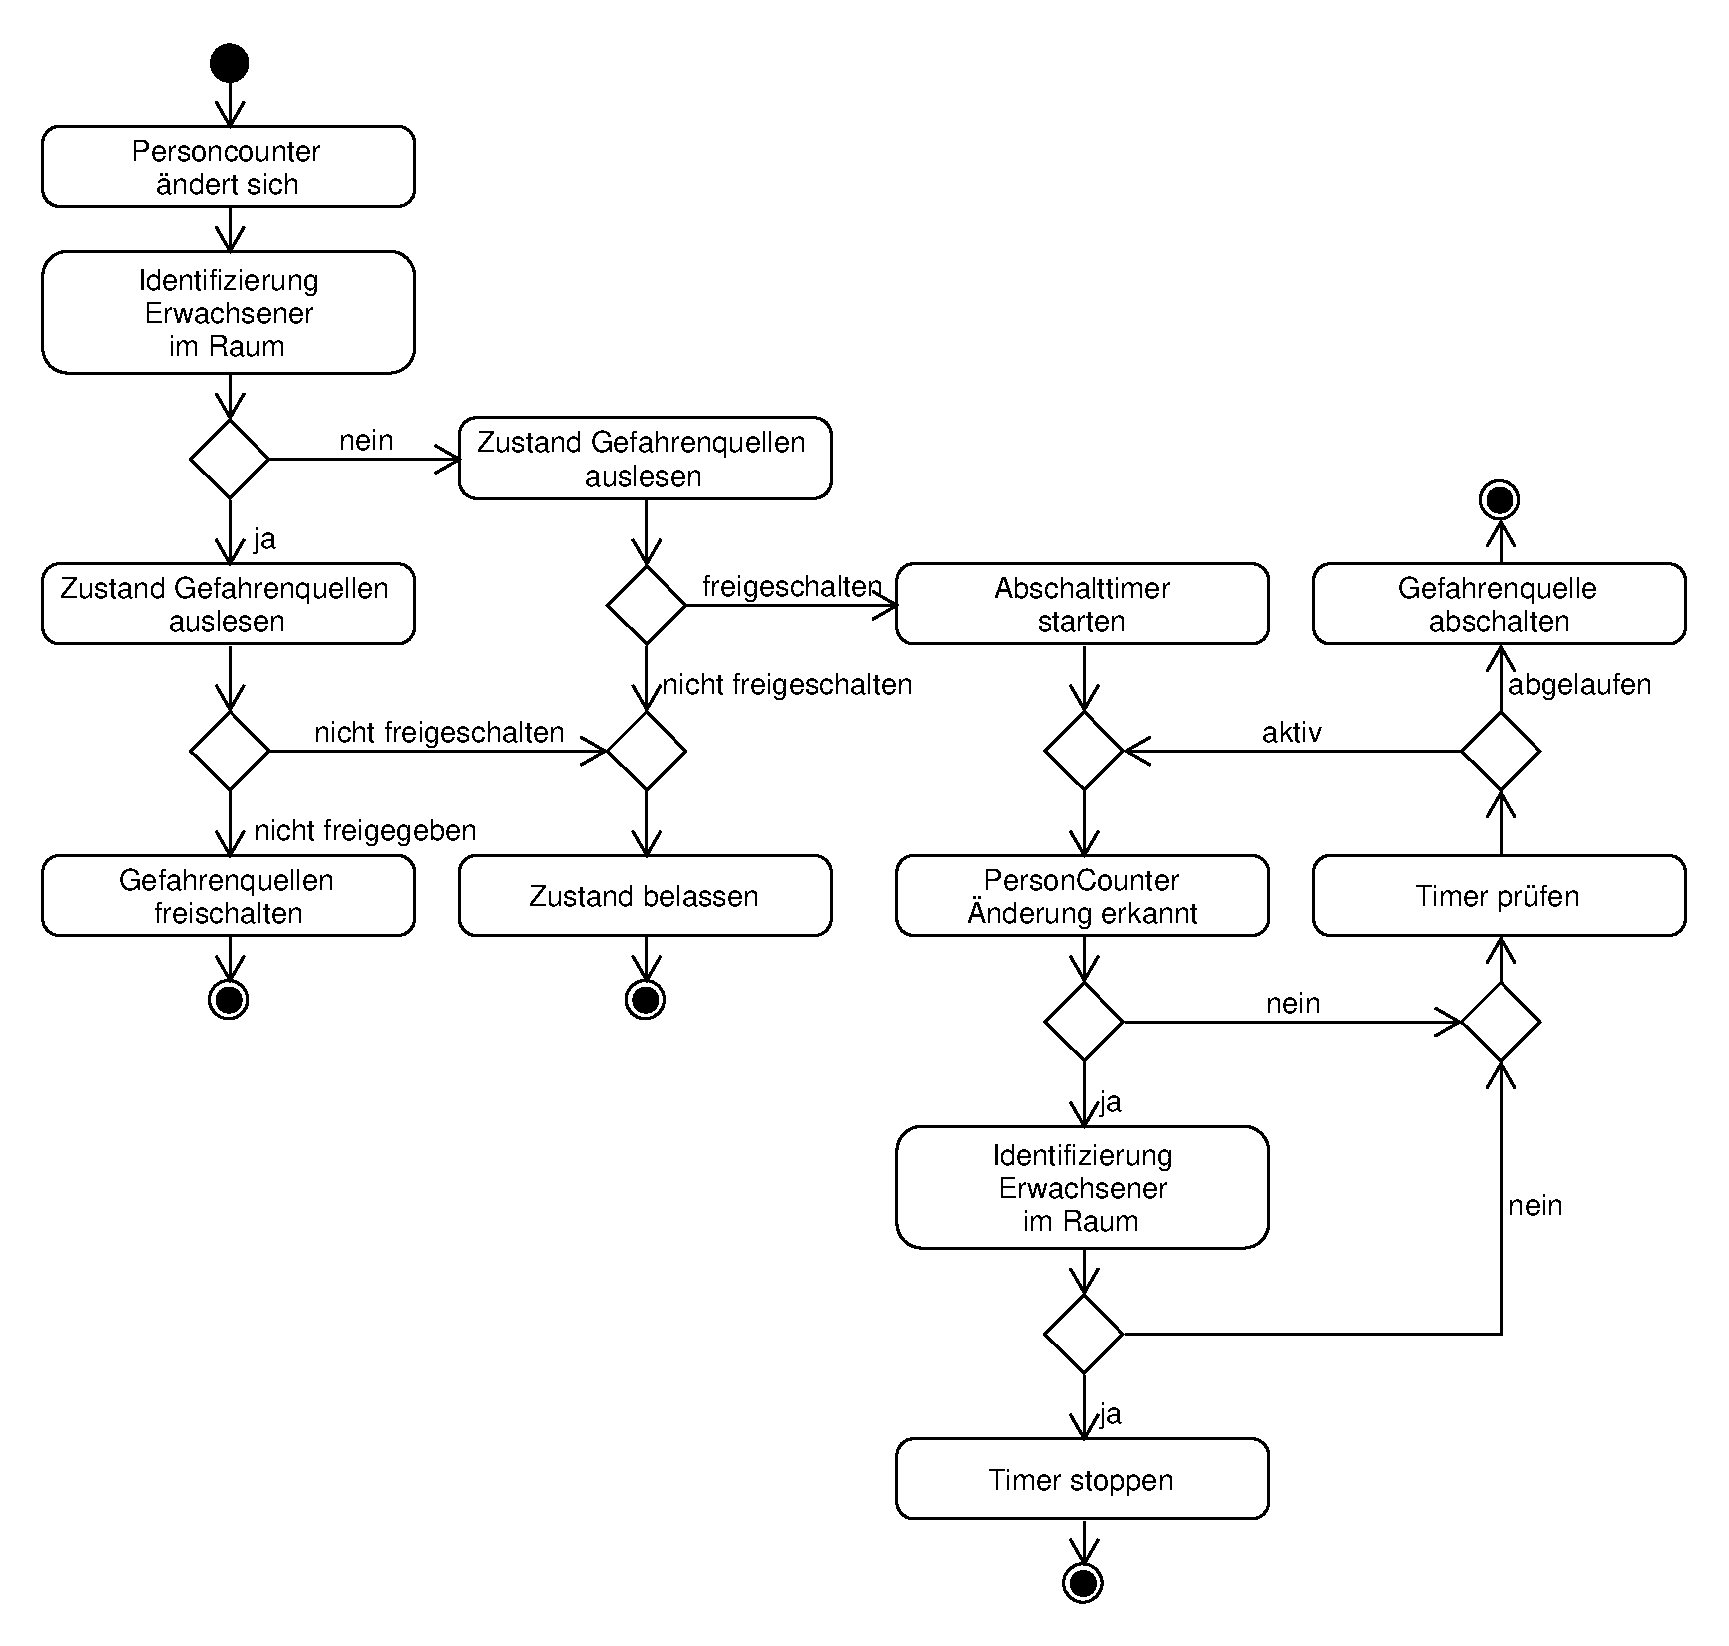
\includegraphics[width=0.9\textwidth]{img/Szenarien/GefahrenquellenAbstellen.pdf}
	\caption{Gefahrenquellen abstellen}
	\label{fig:szenarienGefahrenquellenAbstellen}
\end{figure}


\section{Modulkonzeption}
TODO: allgemeine Beschreibung aller Module, deren Zusammenwirken (Grafik).

\subsection{LockDoorModule}
\emph{von Simon Schwabe}

\subsubsection{Allgemein}
Das LockDoorModule ist der Vermittler für weitere Module im Zusammenhang mit dem Verlassen der Wohnung. Wenn die Wohnung verlassen und abgeschlossen wird, ist die Wahrscheinlichkeit hoch, dass keine weiteren Personen anwesend sind. Allerdings kann die Wohnung auch irrtümlich abgeschlossen werden und es sind noch weitere Personen anwesend. Um solchen Fehlinterpretationen entgegenzuwirken überprüft das LockDoorModule immer, ob wirklich keine Personen erkannt werden und die Wohnung leer steht. Diese Information ist für weitere Module, insbesondere das AlarmModule, relevant und wird über den Event Bus mitgeteilt.

\subsubsection{Funktionsweise}
Die genaue Funktionswese des Moduls wurde im Wesentlichen schon im Abschnitt %TODO beschrieben und modelliert. Das Modell „Abläufe bei Verschließen der Wohnung aus Systemsicht“ %TODO beschreibt das Vorgehen. Die Aktivität „Standby aktivieren“ kann um das Werfen des entsprechenden Events erweitert werden.

Das Szenario enthält keine detaillierte Beschreibung für die Abschaltung des Standby-Modus, da nicht sinnvoll. Für das Modul LockDoor ist es allerdings erforderlich auf die Ankunft von Personen zu reagieren, z.B. um das Alarm-Modul zu benachrichtigen und die Alarmanlage abzuschalten. Die Anzahl der durchzuführenden Aktionen ist überschaubar und wird im Modell %TODO dargestellt.


\subsubsection{Konfiguration}
Bei der Konfiguration des LockDoor muss das Wohnungstürschloss angegeben werden, alternativ kann dafür ein Schalter benutzt werden, der im inneren der Wohnung vor dem Verlassen betätigt wird. 
\begin{itemize}
	\item Schloss/Schalter
	\begin{itemize}
		\item Typ: BinarySwitch
		\item erforderlich: ja
	\end{itemize}
\end{itemize}

\subsubsection{Schnittstellen}
Die Schnittstellen, welche dieses Modul nutzt und bereitstellt, sind von großer Bedeutung. Das Modul an sich implementiert geringe Funktionalität, es ist eine Brücke zwischen den Modulen zur Raumüberwachung auf der einen Seite, und den Modulen für Aktionen bei Verlassen der Wohnung.

LockDoor bietet über den Event Bus eine Schnittstelle zu anderen Modulen. Diese werden benachrichtigt, sobald davon ausgegangen wird, dass keine Person mehr anwesend ist (LockDoorModule\_locked). Die Freischaltung geschieht über ein weiteres Event (LockDoorModule\_unlocked).

Das Modul wird als Singleton angelegt, da für jede Wohnung nur ein Modul zur Überwachung der Wohnungstür erforderlich ist. Das hat zur Folge, dass Events keine Virtual Device Id tragen. Damit ist es für Empfänger einfacher, auf entsprechende Events zu Reagieren.

Für die Überprüfung der Personenanzahl wird die Schnittstelle des Moduls PersonCounter genutzt. Dazu wird für jeden Raum die Anzahl der Personen überprüft.


%\begin{tabularx}{\textwidth}{ X X X }
%	\hline \multicolumn{3}{c}{\textbf{Event Bus - Senden}}  \\ 
%	\hline Event Name 					& Parameter 	& Beschreibung \\ 
%	\hline door\_lock\_module\_locked	& - 			& Tür verschlossen, keine Person anwesend \\ 
%	\hline door\_lock\_module\_unlocked & - 			& Tür geöffnet \\ 
%	\hline 
%\end{tabularx}

\begin{table}
\begin{tabularx}{\textwidth}{
		 >{\hsize=1.25\hsize}X % 40% of 3\hsize 
		>{\hsize=0.5\hsize\centering}X % 30% of 3\hsize
		>{\hsize=1.25\hsize}X % 40% of 3\hsize
		% sum=3.0\hsize for 3 columns
	}	
	\hline
	\textbf{Event Name}					& \textbf{Parameter}	& \textbf{Beschreibung} \\
	\hline LockDoorModule\_locked		& - 					& Tür verschlossen, keine Person anwesend \\ 
	\hline LockDoorModule\_unlocked		& - 			 		& Tür geöffnet \\ 
	\hline
\end{tabularx}
\caption{Event Bus - Senden}
\end{table}


%\begin{longtable}{R{5cm} L{7cm}}
%	\toprule
%	\textit{Option} & \textit{Konfiguration} \\
%	\midrule
%	Feedbackart & Frage \\ [0.25cm]
%	Feedback von & Nutzer mit E-Mail-Adresse für Rückmeldungen \\[0.25cm]
%	Ausführender & Mitarbeiter der Abteilung \glqq Qualitätssicherung\grqq \\[0.25cm]
%	Kategorie & Einordnung in die Kategorie \glqq Mobiles Menü-Bestellsystem\grqq \\[0.25cm]
%	Erklärung & Frage mit Zusatzinformationen zur Menükomponente auf die sich die Frage bezieht \\[0.25cm]
%	\bottomrule	
%	\caption{Beispielkonfiguration des CRM Systems}
%\end{longtable}

\subsubsection{Abhängigkeiten}
\begin{itemize}
	\item PersonCounterModule
	\item TurnOffTimerModule
\end{itemize}
Die entsprechenden Module sind noch nicht beschrieben und genutzte Schnittstellen müssen noch analysiert und auf Nutzungsmöglichkeiten überprüft werden.

Das PersonCounterModule wird zur Überprüfung der Personenanzahl je Raum genutzt. Dazu werden Aufrufe über die ZAutomation-API an das Modul gesendet.

Der TurnOffTimer stellt die eine Schnittstelle zum FeedbackModule her. Durch die zusätzliche Abstraktionsschicht des TurnOffTimers arbeitet das LockDoorModule nicht direkt gegen das FeedbackModul, sondern startet lediglich den Timer. Dieser übernimmt die Kommunikation mit dem FeedbackModule.


\subsubsection{Interne Speicher}
\begin{itemize}
	\item konfiguriertes Türschloss
\end{itemize}

\section{Sensorevaluation}
\begin{itemize}
	\item Ergebnisse der Sensorevaluation (je Sensor)
	\item Was funktioniert wie erwartet/was nicht?
	\item Welche technischen Probleme, lassen sich diese einschränken?
	\item Sind Probleme auf Hardware/Software zurückzuführen?
\end{itemize}

\subsection{Fibaro Wall Plug (FGWPx-102) – Zwischenstecker}

\emph{(von Patrick Hecker)}
\subsubsection{Funktionalität}
\begin{itemize}
	\item ZWave kompatibler Zwischenstecker in Form eines Steckdosenadapters
	\item Steuerung elektrischer Geräte (max. 2,5 kW)
	\item Messung von Wirkleistung und Stromverbrauch
	\item Anzeige über Schaltzustand und Stromverbrauch über Mehrfarben-LED-Ring
	\item Steuerung am Gerät über Taste
\end{itemize}
\subsubsection{Z-Way Elemente}
\begin{itemize}
	\item Fibaro Wall Plug
	\begin{itemize}
		\item Binary Switch
		\item Steuerung des Schaltzustandes
	\end{itemize}
	\item Meter Electric
	\begin{itemize}
		\item Sensor Multilevel
		\item Stromverbrauch in kW
	\end{itemize}
	\item Sensor Power
	\begin{itemize}
		\item Sensor Multilevel
		\item Wirkleistung in W
	\end{itemize}
\end{itemize}

\subsubsection{Konfiguration}

\paragraph{Immer An - Funktion}
\begin{itemize}
	\item Parameter 1:
	\begin{description}
		\item [0] aktiviert,
		\item [1] deaktiviert
	\end{description}
\end{itemize}

\paragraph{Der Zwischenstecker kann auf Z-Wave Netzwerk Alarm reagieren}
\begin{description}
	\item [Parameter 34:] Welcher Alarm soll Reaktion auslösen?
	\begin{description}
		\item [1] genereller Alarm
		\item [2] Rauchalarm
		\item [4] CO Alarm
		\item [8] CO$_2$ Alarm
		\item [16] Temperaturalarm
		\item [32] Überflutungsalarm
		\item [63] auf jeden Alarm reagieren
	\end{description}
	\item [Parameter 35:] Reaktion auf Alarm
	\begin{description}
		\item [0] keine Reaktion,
		\item [1] Schaltzustand ein,
		\item [2] Schaltzustand aus, zyklischer Wechsel (an/aus) jede Sekunde	
	\end{description}
	\item [Parameter 39:] Dauer der Reaktion
	\begin{itemize}
		\item 1 – 65536 Sekunden
	\end{itemize}
\end{description}

\paragraph{Aussenden verschiedener Reports}
\begin{description}
	\item [Parameter 40 - 45] nur bei Änderung des Stromverbrauchs
	\item [Parameter 47] periodisch, ohne Berücksichtigung des Stromverbrauchs
	\begin{description}
		\item [Parameter 40:] Sofortiger Report über Stromverbrauch (W)
		\begin{itemize}
			\item 1 – 100 \%
		\end{itemize}
		\item [Parameter 42:] Standardmäßiges Aussenden von Reports über den Stromverbrauch
		\begin{itemize}
			\item 1 – 100 \%
		\end{itemize}
		\item [Parameter 43:] Zeitintervall zum Senden eines Reports über den Stromverbrauch
		\begin{itemize}
			\item 1 – 254 Sekunden (bezieht sich auf Parameter 42)
		\end{itemize}
		\item [Parameter 45:] Änderung in der Stromaufnahme durch gesteuerte Geräte (kWh)
		\begin{itemize}
			\item 1 – 254 (0,01 – 2,54 kWh)
		\end{itemize}
		\item [Parameter 47:] Zeitintervall zwischen den Reports über die momentane Wirkleistung und den Stromverbrauch
		\begin{itemize}
			\item 1 – 65534 Sekunden
			\item Erklärung: Report im Zeitintervall, ohne Änderung im Verbrauch!
		\end{itemize}
		\item [Parameter 49:] Messen des Eigenstromverbrauchs des Wall Plug Moduls
		\begin{description}
			\item [0] keine Einbeziehung des Eigenstromverbrauchs
			\item [1] inklusive Eigenstromverbrauch
		\end{description}
	\end{description}
\end{description}

\paragraph{Einstellungen zu Assoziationsgruppe 2}
\begin{description}
	\item [Parameter 50:] Unterer Leistungsschwellwert
	\item [Parameter 51:] Oberer Leistungsschwellwert
	\item [Parameter 52:] Konfiguration des Verhaltens beim Überschreiten der festgelegten Leistungsschwellwerte
\end{description}

\paragraph{Farbeinstellungen}
\begin{description}
	\item[Parameter 60:] Leistungsschwellwert für violettes Blinken
	\begin{itemize}
		\item 1000 – 32000 (100 – 3200 W)
	\end{itemize}
	\item [Parameter 61:] LED-Ring-Farbe im Einschaltzustand
	\item [Parameter 62:] LED-Ring-Farbe im Ausschaltzustand
	\item [Parameter 63:] LED-Ring-Farbe bei Z-Wave-Alarmmeldung
	\item [Parameter 61 - 63:] Farbwerte
	\begin{description}
		\item [1] White
		\item [2] Red
		\item [3] Green
		\item [4] Blue
		\item [5] Yellow
		\item [6] Cyan
		\item [7] Magenta
		\item [8] Farbe aus
	\end{description}
\end{description}
Weitere Informationen (auch technische Details) sind dem Handbuch zu entnehmen.


\subsection{Aoetec Multisensor Sensor}
\emph{(von Alexander Keller)}

\subsubsection{Allgemein}
Im Bereich Smarthome hat man eine riesige Auswahl von verschiedenen Sensoren. Je nach Bedarf bieten die Multisensoren verschiedene Funktionalitäten welche Bewegungen, Raumtemperatur, Licht oder andere registrieren können. Der Aeotec Sensor erfasst 6 verschiedene Messwerte. Die Sensoren messen Raumtemperatur, Lichtstärke, Luftfeuchtigkeit, Bewegung, \gls{uv}-Sensor und Vibration. Diese Werte überträgt der Multisensor mit einer drahtlosen Kommunikationsschnittstelle namens Z-Wave.

In unserem Projekt kommt dieser Sensor zum Einsatz, um das Alarm Modul, Personenidentifikationsmodul und Gefahrenmodul mithilfe seiner Sensortechnik zu unterstützen. Durch seine durchaus komplexe Konfigurationsmöglichkeit kann der

//TODO: wie geht's hier weiter?

\subsubsection{Konfigurationsmöglichkeiten}
Nachdem man das Gerät erfolgreich im Z-Way Home Center hinzugefügt hat, besteht die Möglichkeit den Multisensor über die Expert-UI zu konfigurieren. 

\begin{figure}[h!]
	\centering
	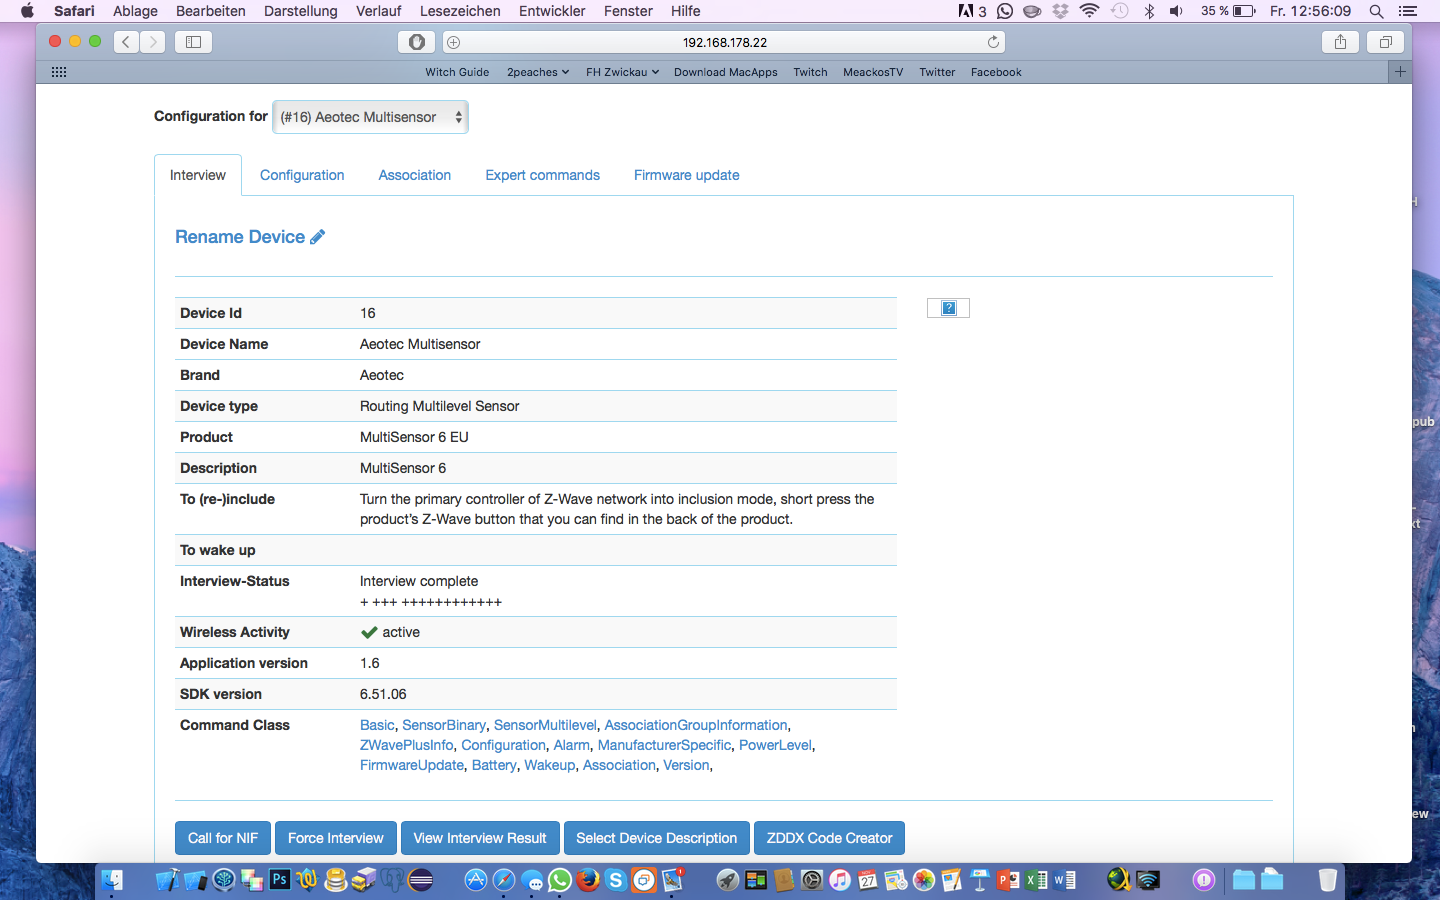
\includegraphics[width=0.9\textwidth]{img/Sensorevaluation/AeoScreenshot.png}
	\caption{Übersichtsseite des Aeotec Multisensor}
	\label{fig:sensorenAeoScreenshot}
\end{figure}

Der Z-Way Server erstellt automatisiert eine Übersichtsseite nachdem der Sensor erfolgreich hinzugefügt wurde. In diesem Reiter besteht die Möglichkeit das Gerät umzubenennen, Netzwerkstatus abzurufen, \gls{sdk} Version.

Im Reiter „Configuration“ findet man alle Einstellungsmöglichkeiten die der Sensor bietet. In der nachfolgenden Tabelle, finden sie alle Konfigurationsoptionen.

\begin{table}
	\begin{longtabu} to \linewidth {
			>{}X
			>{}X
			>{}X
		}	
		\hline
		\textbf{Name}							& \textbf{Optionen}		& \textbf{Beschreibung} \\
		\hline 
		Wake Up 10 Minutes when	batteries are inserted	
				& No \newline Yes				
						& Der Sensor "`erwacht"' alle 10 Minuten, wenn Batterien eingelegt sind. \\ 

		\hline 
		On Time									& X Minuten	 		& Wie lang sollen die verschiedenen Sensoren den aktuellen Wert speichern bevor diese aktualisiert werden \\ 
		\hline
		Enable/Disable the function of motion Sensor &
				(0) disable \newline
				(1) enable, the current PIR sensitivity level=1. (minimum level) \newline
				(2) enable, the current PIR sensitivity level = 2. \newline
				(3) enable, the current PIR sensitivity level=3. \newline
				(4) enable, the current PIR sensitivity level=4. \newline
				(5) enable, the current PIR sensitivity level=5. (maximum level) \newline &
						Es besteht die Möglichkeit den Bewegungssensor zu deaktivieren \& die Intensität einzustellen \\
		\hline
		Motion Detection &
				(1) Send Basic Set CC. \newline
				(2) Send Sensor Binary Report CC. &
						Welchen Standard soll der Aeotec Sensor sende, wenn der Bewegungssensor ausgelöst wurde \\
		\hline
		Low Batterie Value &
				X \% &
						Ab welchen prozentualen Wert soll der Sensor bescheid geben, wenn der Batteriestand niedrig ist. \\
		\hline
		Reports for Parameter 41 – 44 &
				(0) disable \newline
				(1) enable &
						Diese Funktionalität dient dazu um bestimmte Schwellenwerte in bestimmten Zeitabständen zu an den Z-Way Server zu senden. (Netzwerktraffic) \\
		\hline
		Humidity Automatic Report &
				X Schwellenwert &
						Festlegen eines Schwellenwertes für den Feuchtigkeitssensor \\
		\hline
		Luminance Automatic Report &
				X Luminanz &
						Festlegen eines Schwellenwertes für den Lichtsensor \\
		\hline
		Battery Automatic Report &
				X Prozent &
						Festlegen eines Schwellenwertes für die Batterieänderung \\
		\hline
		Threshold change in ultraviolet to induce an automatic report. &
				X Schwellenwert &
						Festlegen eines Schwellenwertes für Ultra Violettes Licht \\
		\hline
		Low Temperature Alarm Report &
				(0) Disable to send the alarm report of low temperature \newline
				(1) Enable to send the alarm report of low temperature &
						 Bericht wenn die Temperatur unter 15 Grad fällt. \\
						
	\end{longtabu}
	\caption{Config des Sensors}
\end{table}

